\section{Autonomus Driving System Architecture}\label{sec:design-avSystemArchitecture}
This section will describe the proposed overall architecture for the autonomous driving system developed in this project. An illustration of this can be seen in \autoref{fig:design-avs-overallArchitecture}. The system is divided into four phases, namely Data Collection, Training, Inference and Steering, where the former two takes place offline and the ladder two takes place during the live run of the system, where the vehicle is driving by itself.

\begin{figure}[H]
    \centering
    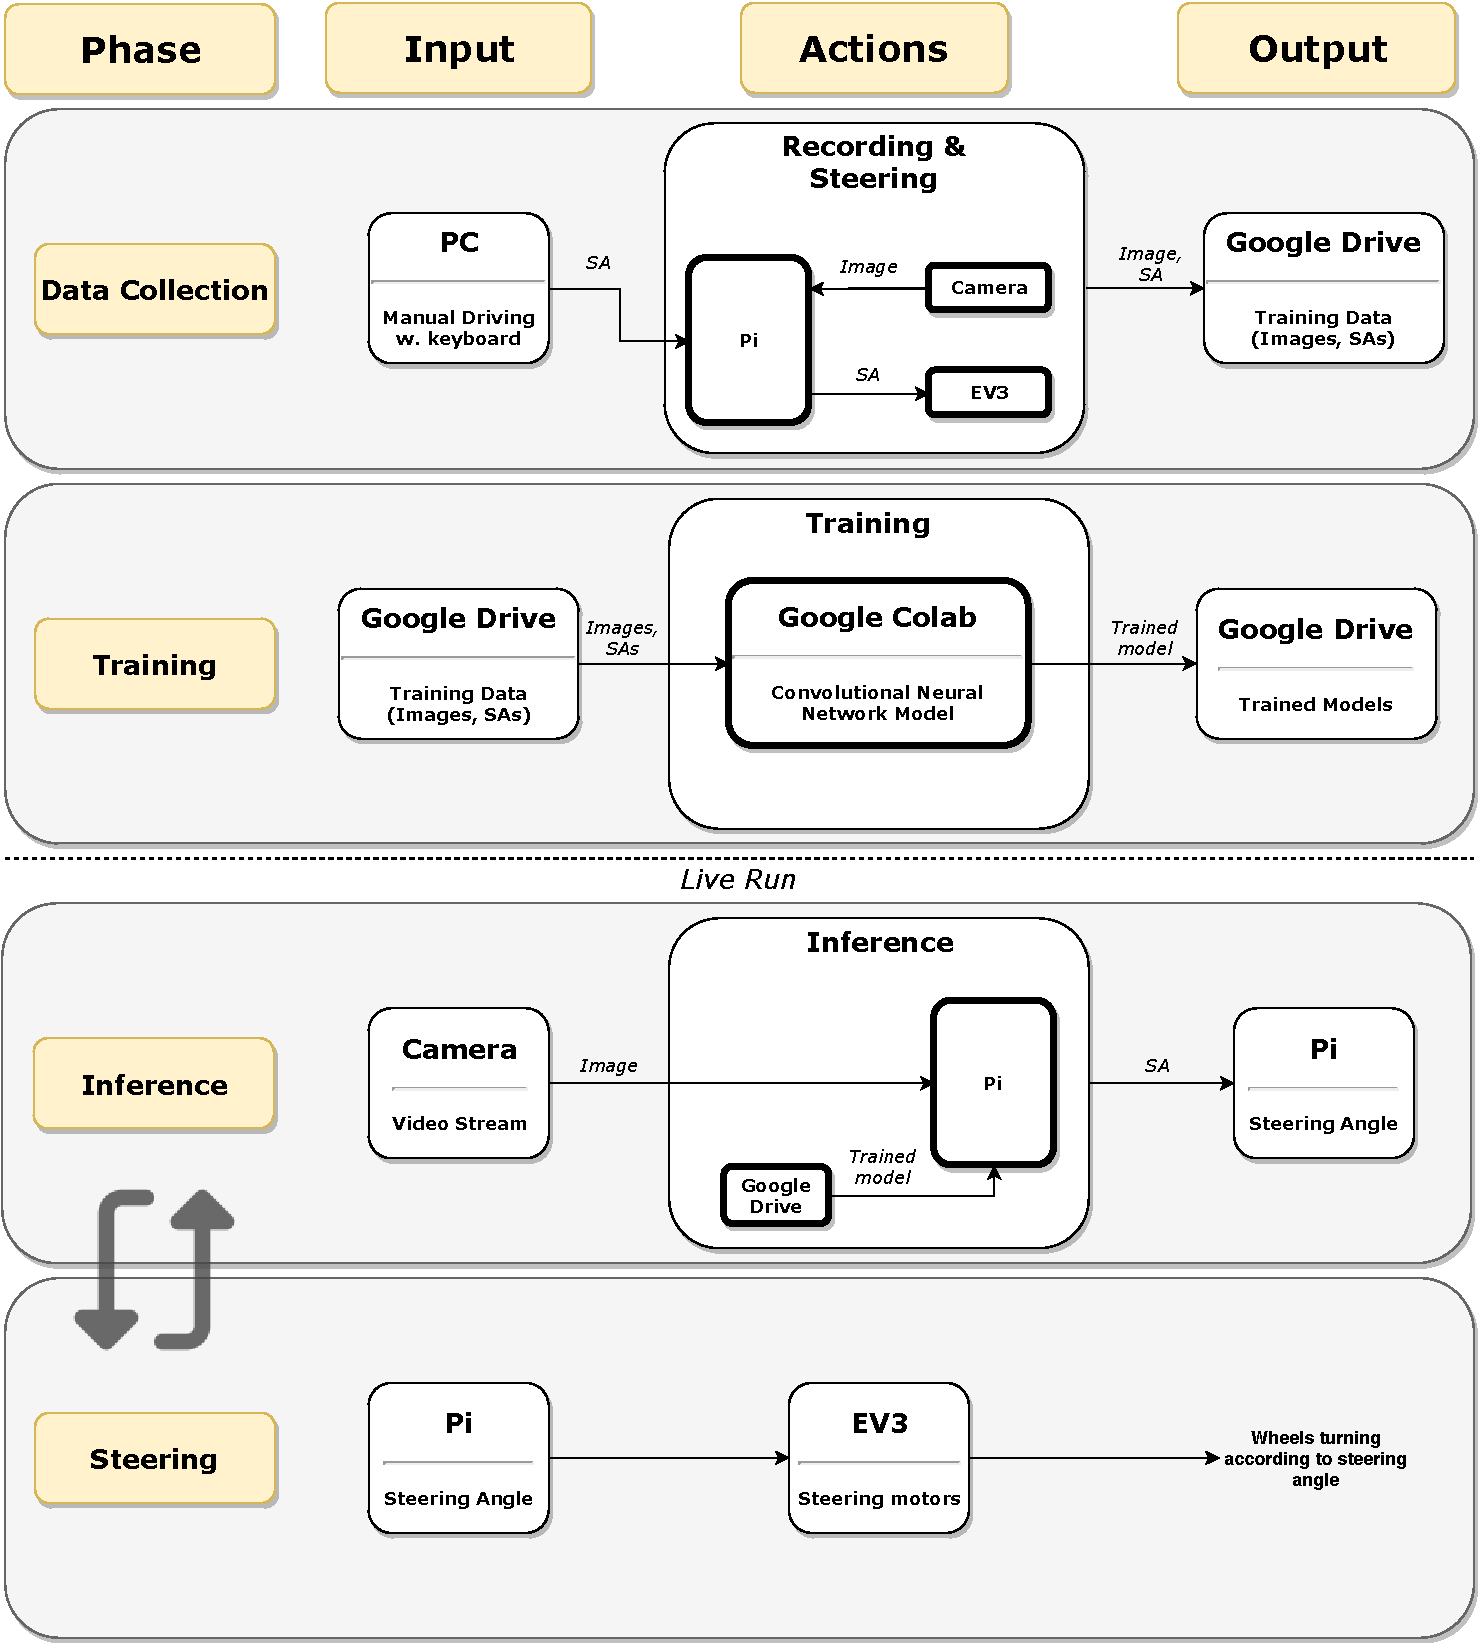
\includegraphics[width=\textwidth]{images/design/overall-system-architecture.pdf}
    \caption{Overall architecture of the autonomous driving system. SA is short for steering angle.}
    \label{fig:design-avs-overallArchitecture}
\end{figure}

The required data to train a convolutional neural network,will be gathered by driving the vehicle manually with a pc connected to the raspberry pi, which in turn is connected to the EV3 and a camera. This allows for passing steering angles to the ev3 through the keyboard on the pc, while obtaining images from the videostream on a camera. These images can then in turn be labeled with the steering angle and stored in Google Drive and constitutes the training data for that particular run.

In order to train the model, it was decided to use Google Colab, which is a common cloud computing service for training artificial neural network models. The idea is to setup Google Colab to automatically gather the training data from Google Drive, in order to train the convolutional neural network model that will be implemented and in turn store that trained model back in Google Drive.

For the live run, the Inference and Steering phases, should run iteratively, where the Camera's video stream gives an image to the Pi as in the manual run. Now however,the steering angle should be obtained through inference on the trained model on the pi with that image, instead of manually from the PC. This steering angle should then be used in the Steering phase by the Pi to instruct the EV3 to steer its motors accordingly, resulting in the wheels being turned by that angle.